% !TeX spellcheck = de_DE
\documentclass[.../Dokumentation.tex]{subfiles}
\begin{document}
    \subsection{Hard- und Software}
    \label{sec-ita3-hardware}
    \subsubsection*{Visualisierung}
    Die erste funktionsfähige Fahrzeugsoftware bildet die Grundlage für die Implementation der Visualisierung. Die Basis hierfür ist das Webframework \emph{Flask}. Mit diesem wird eine REST-Schnittstelle entworfen, welche die gesendeten Fahrzeugdaten empfängt. \\\\
    In einer Konfigurationsdatei werden die verschiedenen Fahrzeugtypen und die zugehörigen Fahrzeugeigenschaften gespeichert. Die Eigenschaften umfassen eine eindeutige ID, den Namen des Typs, den Radius der Räder, die Anzahl an Magneten in diesen und die verursachte Umweltverschmutzung pro gefahrenem Zentimeter. Somit muss der Programmcode auch bei zukünftigen Änderungen nicht angepasst werden und verschiedene Fahrzeugtypen können einfach eingefügt und abgebildet werden.\\\\
    Wenn ein Fahrzeug sich bewegt, sendet es die Anzahl an erfassten Magnetkontakten und die ID des Fahrzeugs an den Raspberry Pi. Dieser berechnet im ersten Schritt mithilfe der spezifizierten Werten in der Konfigurationsdatei die verursachte Umweltverschmutzung. Das Ergebnis wird im zweiten Schritt mit einem Zeitstempel versehen und gespeichert. Da die Messwerte nur wenige Sekunden aktuell sind und keine persistente Speicherung benötigen, wird keine Datenbank aufgesetzt. Die Werte werden lediglich im RAM gespeichert.\\\\
    Das Programm startet zu Beginn einen weiteren Thread. Dieser ist für die Steuerung der Hardware-Komponenten verantwortlich. Hierfür wird alle $x$ Sekunden eine Funktion aufgerufen. Diese iteriert zuerst über alle gespeicherten Verschmutzungseinträge und löscht die veralteten. Hierfür wird die aktuelle Systemzeit und der Zeitstempel des Eintrags verglichen. Die Gültigkeit von diesen kann in der Konfigurationsdatei angepasst werden. Danach werden die verbleibenden, gültigen Werte addiert und ergeben die gesamte Verschmutzung. Diese wird an die einzelnen Hardware Komponenten weitergeleitet. Für die Steuerung der Servo Motoren wird ein PWM Signal verwendet. Mit der zuvor berechneten Verschmutzung wird die Rotation von diesen bestimmt. Dabei entspricht $0 \degree$ keiner und $180 \degree$ der maximalen Verschmutzung. Für die LEDs wird der WS2812B LED-Streifen der Firma Adafruit verwendet. Dieser wird über die dazugehörige Python Bibliothek angesteuert. Je nach Verschmutzung setzt sich die Farbe aus grün und rot zusammen. Die hierfür verwendet Schaltung ist in Abbildung \ref{fig-tree_iteration3_wiring} dargestellt. 
       	\begin{figure}[H]
    	\begin{center}
    		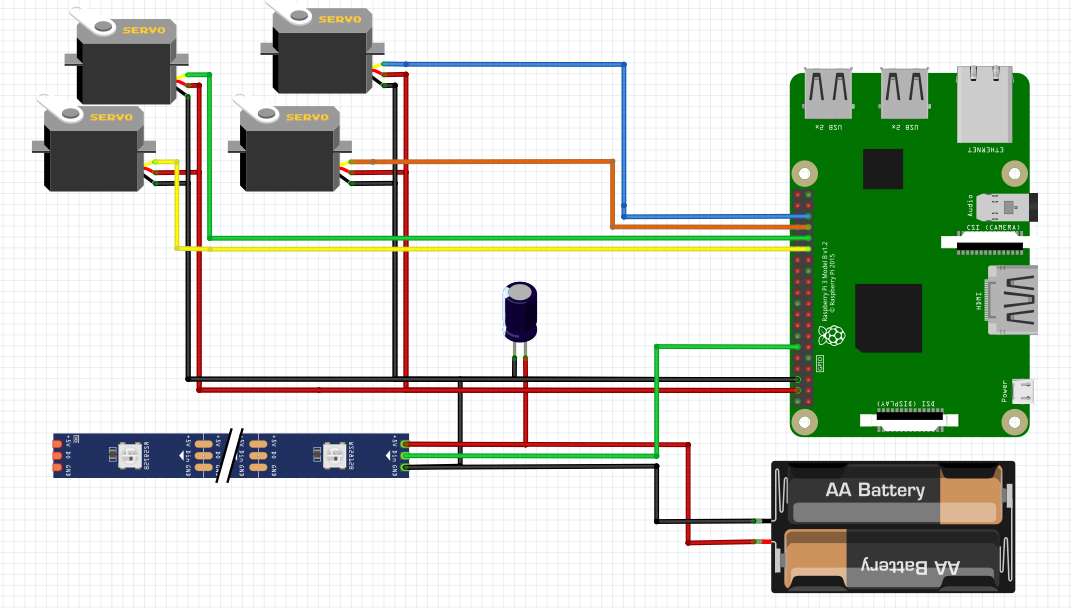
\includegraphics[
    		width=0.7\linewidth,
    		]{imgs/tree_wiriring_iteration3.PNG}
    		\caption{Schaltung für den Baum}
    		\label{fig-tree_iteration3_wiring}
    	\end{center}
    \end{figure}
    \noindent
   	Diese enthält zusätzlich einen Kondensator und eine Schnittstelle für eine externe Stromversorgung. Der Kondensator soll Schwankungen der Spannung ausgleichen. Das Netzteil wird verwendet, da der Raspberry Pi nicht genug Strom für die LEDs bereitstellen kann. Mit der vorgestellten Schaltung kann das externe Netzteil zusätzlich den Raspberry Pi über den $5V$-Pin mit Strom versorgen. Somit wird nur ein Netzteil für alle Komponenten  benötigt.
   	
   	\subsubsection*{Fahrzeug}
   	Beim Testen der Visualisierung mit der Fahrzeugschaltung ist ein Problem aufgetreten. Ist das Fahrzeug mit einem USB Kabel an einen Computer angeschlossen, funktioniert die Sensorerkennung. Wird diese nur mit dem Akku betrieben, können keine Sensorwerte erkannt werden. Beim Ausmessen der verfügbaren Spannung zeigt sich, dass im Betrieb mit dem Akku nur $3.3V$ an dem $5V$-Pin verfügbar sind. Wie in Kapitel \ref{sec-ita1-hardware} beschrieben, benötigt der Hall-Sensor mindestens $3.7V$.\\\\
   	Zum Lösen dieses Problems muss die Spannung angehoben werden. Der erste Lösungsansatz ist ein \emph{Logic-Level-Converter}, welcher zwischen dem Sensor und dem Arduino eingebaut werden kann. Dieser kann Signale in bidirektionaler Richtung zwischen zwei Spannungen, wie zum Beispiel $5V \longleftrightarrow 3.3V$, wandeln. Das Problem hierbei ist, dass an einem Pin des Moduls eine $5V$ Spannung angelegt werden muss, welche nicht verfügbar ist.\\
   	Der zweite Ansatz ist das Verwenden eines $Step-Up Boost-Converters$, mit welchem das Problem erfolgreich gelöst werden kann.
   	Dieses akzeptiert eine Eingangsspannung zwischen $2-24V$ und hat eine Ausgangsspannung von $5-28V$. Die Ausgangsspannung kann mit einem Potentiometer eingestellt werden. Die Schaltung des Fahrzeugs wird mit diesem Modul abgeändert. Die neue Version ist in Abbildung \ref{fig-hardware-car-iteration3} dargestellt.
   	\begin{figure}[H]
   		\begin{center}
   			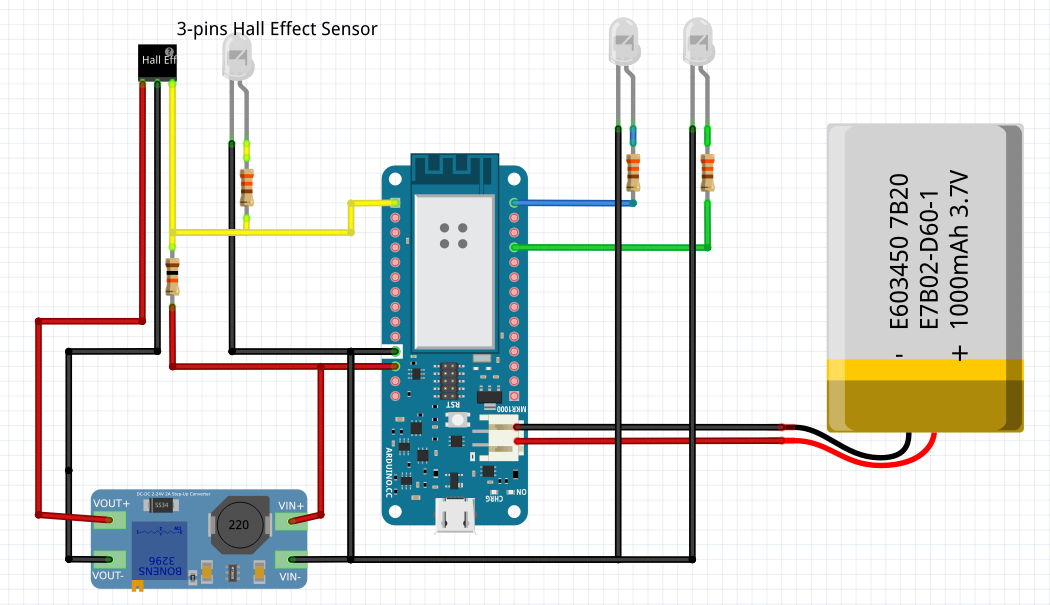
\includegraphics[
   			width=0.7\linewidth,
   			]{imgs/car_wiring_iteration3.png}
   			\caption{Schaltung ein Fahrzeuge mit Boost-Converter}
   			\label{fig-hardware-car-iteration3}
   		\end{center}
   	\end{figure}
   \noindent
   	Der $+$- und $GND$-Pin des Sensors werden an den Output des $Step-Up Boost-Converters$ angeschlossen, welcher auf $5V$ eingestellt wird. Die benötigte Eingangsspannung für das Modul wird vom $3.3V$-Pin des Arduinos geliefert. Somit funktioniert die Schaltung sowohl im Betrieb mit einem USB-Kabel als auch mit einem Akku. 
    
    
\end{document}